%% Options:

%% twocolumn : Two column layout.
%% hf: enable header and footer.
\documentclass[twocolumn]{ceurart}

%%
%% One can fix some overfulls
\sloppy

%%
%% Minted listings support 
%% Need pygment <http://pygments.org/> <http://pypi.python.org/pypi/Pygments>
\usepackage{minted}
%% auto break lines
\setminted{breaklines=true}

\begin{document}

\copyrightyear{2023}
\copyrightclause{
    Copyright for this paper by its authors.
    Use permitted under Creative Commons License Attribution 4.0 
    International (CC BY 4.0).
}

\conference{
    ITAT'23: Information technologies -- Applications and Theory
    September 22--26, 2023, Tatranské Matliare, Vysoké Tatry
}

\title{Prefix-free graphs and suffix array construction in sublinear space}

\author[1]{Andrej Baláž}[
    orcid=0000-0001-0002-0003,
    email=andrejbalaz001@gmail.com,
]
\cormark[1]

\author[1]{Alessia Petescia}[
    orcid=0000,
    email=alessia@gmail.com,
]

\address[1]{
    Department of Applied Informatics,
    Faculty of Mathematics, Physics and Informatics,
    Comenius University, Bratislava, Slovakia
}

% Footnotes
\cortext[1]{Corresponding author}

%%
%% The abstract is a short summary of the work to be presented in the
%% article.
\begin{abstract}
  Recently, many graph structures for computational pangenomics were proposed.
  In order to be useful, these graph structures need to implement several
  operations such as efficient construction from many complete genomes,
  mapping of short and long read.
  These basic bioinformatics operations are well studied on sequential data,
  and together with data structures such as suffix trees, suffix arrays and 
  burrows wheeler transform allow high performance.
  Attempts to implement these operations on graphs brings with it many complications
  since these date structures are not easily obtainable for graphs.
  In this work, we introduce prefix-free graphs, a pangenomic data structure
  allowing to obtain the well known data structures from stringology in graph
  settings, which in turn allows for many efficient operations on pangenomes.
\end{abstract}

%%
%% Keywords. The author(s) should pick words that accurately describe
%% the work being presented. Separate the keywords with commas.
\begin{keywords}
  pangenome \sep
  suffix array
\end{keywords}

%%
%% This command processes the author and affiliation and title
%% information and builds the first part of the formatted document.
\maketitle

\section{Introduction}
Suffix array is a data structure used in many fields, such as stringology,
bioinformatics, and... .
Particularly in bioinformatics, it is used as part of FM index, which in turn
is used for read mapping.
Recently, a new paradigm in bioinformatics was formed, moving from a single
reference genome to a pangenome.
The term pangenome was first used by \citet{tettelin2005genome} in 2005 during the
resequencing experiments on streptococcus.
Since then, the definition of a pangenome has shifted to any set of sequences
analysed jointly \cite{computational2018computational}.
Nevertheless, most pangenomes consist of highly related sequences and thus are
highly repetitive.
This leads to representation of pangenomes as graphs, where similar genome
regions are represented by a single node and the nodes are conected to paths
representing the original sequences.
Several approaches of pangenomic graph construction exist, such as variation
graphs \cite{church2015extending}?, cactus graphs \cite{paten2011cactus}, 
Wheeler graphs \cite{gagie2017wheeler} ...
Most of these approaches require an initial local alignment of similar regions,
which makes them computationally expensive.
Here we present a new class of graphs, prefix-free graphs, which are easy to
construct and provide a way how to efficiently index them to allow pattern 
search queries.
Pangenomes introduced by...
In computational pangenomics...
Repetitive datasets...
Graph pangenomes and textual pangenomes...
Prefix-free parsing is a technique...
Prefix-free graphs play an important role in improving space
complexity of several efficient algorithms, but are never the concept is never
framed as a pangenomic data structure.
We think that separating and clearly defining this data structure can lead to
more advancements...
Our contribution is in defining a data structure called prefix-free graphs and
showing how this data structure can be used to generate suffix array in
sublinear space.
Furthermore, we implemented two binaries for an easy construction of prefix-free
graphs from a set of sequences, and from a graph in gfa format.
Furthermore, we implemented rust library for working with prefix-free graphs.
This library contains an iterator, which can be directly used to generate the 
suffix array in sublinear space.

\section{Prefix-free graphs}
% some intro?
The idea of prefix-free graphs is inspired by rsync \cite{kornblum2006identifying}.
%% Context-triggered piecewise hashing (CTPH) is a technique for parsing
%% strings into blocks such that long repeated substrings are parsed the same
%% way (except possibly at the beginning or end of the substrings).

% what are prefix-free graphs
Given a set of sequences representing a pangenome, we can partition each
sequence into \emph{segment}s.
These segments form nodes of the prefix-free graph.
The edges of a graph represent the adjacencies of the segment pairs, which are 
present in the original strings.
The adjacent segments are overlapping by a fixed number of characters $k$.
We will call these $k$-sized overlaps triggers.
Another important feature of the segments is that they contain triggers only at
the start or at the end of a segment.
This feature guarantees that the set of segments is prefix-free, i.e. no
segment is a prefix of another segment.

\begin{figure}
    \centering
    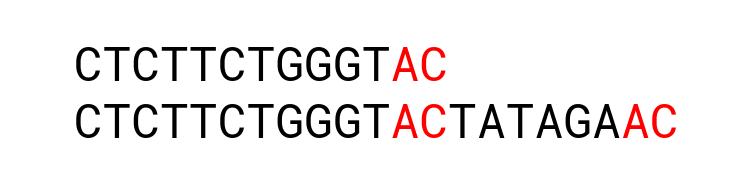
\includegraphics[width=\linewidth]{images/prefixfree_proof.png}
    \caption{Visual proof that the trigger words induce prefix-free segments.}
    \label{fig:proof}
\end{figure}

% how to construct prefix free graphs
To illustrate how to partition the sequences into segments consider a set of
strings $S = {TACTACGTACT, TCGTACTACT, TCGTCGTACTACT}$.
Next, assume we will partition the sequences using a set of trigger words 
$T = {AC, CG}$.

In stringology, strings are often flanked by so called \emph{sentinel} = $\$$.
In our case, we need to append $k$ sentinels to the sequences.
The reasons for doing so will become clear in the suffix array construction section.

Then, using a sliding window we can scan through the sequences and each time we
encounter a trigger word, we create a new segment from the start of the previous
trigger word to the end of the current trigger word.
Two special cases happen at the beginning of a sequence, when no previous
trigger was encountered, and at the end.
In the former case, the segment starts simply at the start of a sequence and in
the later case the segment ends at a sequence end.

During the sequence scan, each unique segment is assigned an ID.
The original sequence can then be represented as a list of IDs, also called 
\emph{path}s.

The result of this procedure is a set of segments and a list of paths.
In the previous example, the segments are ${ TAC, ACTAC, ACG, CGTAC, ACT\$\$, TCG, CGTCG }$
and the paths are $[  ]$.

Because each segment is represented in a set $S$ only once, the sum of lengths
of segments is usually much smaller than the length of original sequences.

This set of segments, together with the list of paths are already a prefix-free
graph, but in order to be useful for the next part, we need to normalize it.
By normalizing, we mean to sort the segments lexicographically and relabel the
paths accordingly.
This will give us a list of segments and a list of paths which can be directly
represented in the GFA format as shown in the Figure \ref{fig:gfa}.

\begin{figure}
    \centering
    % 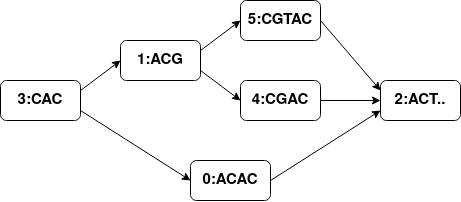
\includegraphics[width=\linewidth]{images/pfg.drawio.png}
    % 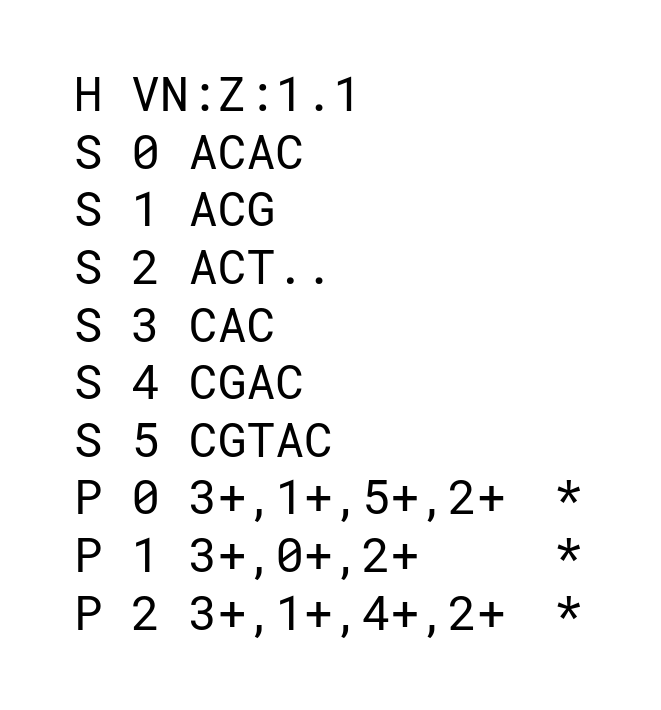
\includegraphics[width=0.5\linewidth]{images/pfg_gfa.v2.png}
    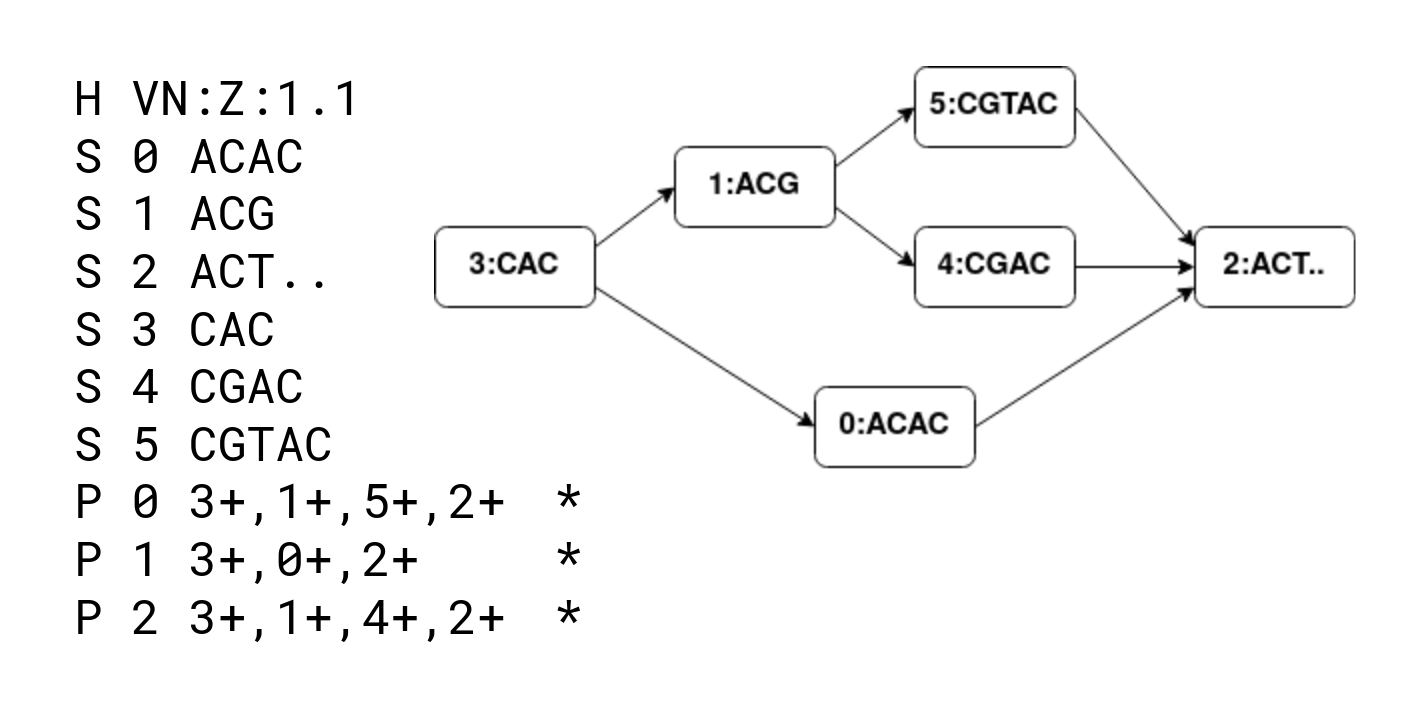
\includegraphics[width=\linewidth]{images/pfg_gfa.v3.png}
    \caption{Prefix-free graph in GFA format. Link lines omitted for brevity.}
    \label{fig:gfa}
\end{figure}

% add graph figure

The reconstruction of the original sequence can then be done by expanding 
the particular path, ignoring last $k$ characters of each segment.

\section{Suffix array construction}
Suffix array is a permutation of string positions which lexicographically
sorts the suffixes of the string starting at that position.
It is extremely powerful data structure with many applications in efficient
algorithms on strings.
Enhanced by additional data structures, such as for example longest common
prefix (LCP) array, it can fully substitute suffix tree and solve problems,
such as exact pattern matching, repeat finding, maximum exact matching (MEM)
finding, document retrieval and many more.

There exists several algorithms for suffix array construction in linear time
\cite{} with several practical implementations \cite{}.
Altough their time complexity is linear, these algorithms become bottlenecks in
some application due to their linear space complexity.
This is especially relevant in pangenomics, where the datasets often do not fit
in the memory.
Nonetheless, as we shown in previous sections, prefix-free graphs can represent
the pangenome in substantialy smaller space and therefore can fit in computer
memory.

Here we show another crucial advantage of prefix-free graphs - their ability to
output the suffix array of the original string iterativelly.
This allows us to generate the suffix array one-by-one with the possibility
to compress or use in subsequential computations directly, giving us the ability
to use the rich theory of suffix arrays without ever storing them.

\subsection{Iterator preparation}
In order to prepare the prefix-free graph to generate the suffix array of
original pangenome we need to create several data structures.
First, we concatenate all the prefix-free segments into a single string using
a separator $\#$ and append a sentinel $\$$.
We will call this concatenation \emph{segment join}.
An example of a segment join is in the Figure \ref{fig:ids_and_positions}.

Next, for the segment join we calculate the suffix array and the LCP array.
For this we can use the linear time, linear space algorithms mentioned previously,
since the segment join is usually much smaller than the original pangenome.

Next, for each suffix of a segment join, we need to calculate the corresponding
segment ID and the segment position.
These two arrays represent the current suffix of a segment join starts with a
particular segment and the position in this segment.
This can be computed using an inverse permutation of a suffix array of a segment
join in linear time.
To illustrate the procedure, consider the segment join of our running example from
Figure \ref{fig:ids_and_positions}.
Each position of the join can be assigned a segment ID and a position in current
segment by linearly iterating the segment join and incrementing ID and position
accordingly.
Then, applying the inverse permutation of a suffix array to these arrays will
change the order of computed values in a way corresponding to the sorted suffixes.
The Table \ref{tab:suffix} shows the resulting suffix array, LCP array,
segment ID array and segment position array.

\begin{figure}
    \centering
    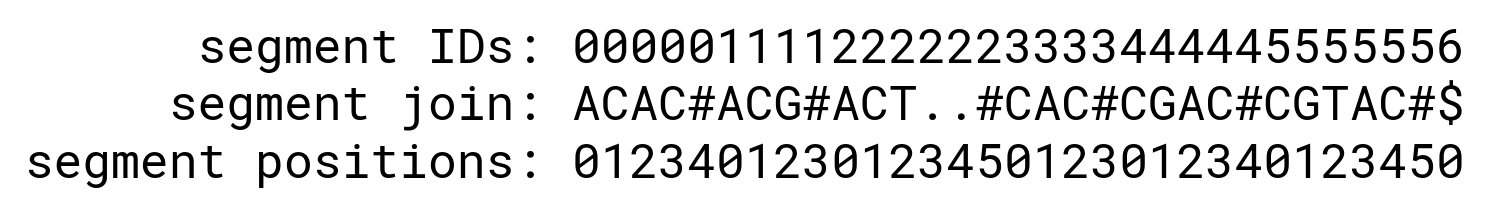
\includegraphics[width=\linewidth]{images/ids_and_positions.png}
    \caption{
        Segment IDs and segment positions of a segment join. Permuting these
        according to the inverse permutation of a suffix array results in 
        segment ID array and segment position array shown in the Table \ref{fig:segment_sa}.
    }
    \label{fig:ids_and_positions}
\end{figure}

\begin{table*}
    \caption{Suffix table}
    \label{tab:suffix}
    \begin{tabular}{rrrrrl}
        \toprule
        i & SA[i] & LCP[i] & ID[i] & pos[i] & suffix[i..]\\
        \midrule
         0  & 30 & -1 & 6 & 0 & \texttt{\$}                                     \\
         1  & 29 &  0 & 5 & 5 & \texttt{\#\$}                                   \\
         2  &  4 &  1 & 0 & 4 & \texttt{\#ACG\#ACT..\#CAC\#CGAC\#CGTAC\#\$}     \\
         3  &  8 &  3 & 1 & 3 & \texttt{\#ACT..\#CAC\#CGAC\#CGTAC\#\$}          \\
         4  & 14 &  1 & 2 & 5 & \texttt{\#CAC\#CGAC\#CGTAC\#\$}                 \\
         5  & 18 &  2 & 3 & 3 & \texttt{\#CGAC\#CGTAC\#\$}                      \\
         6  & 23 &  3 & 4 & 4 & \texttt{\#CGTAC\#\$}                            \\
         7  & 13 &  0 & 2 & 4 & \texttt{.\#CAC\#CGAC\#CGTAC\#\$}                \\
         8  & 12 &  1 & 2 & 3 & \texttt{..\#CAC\#CGAC\#CGTAC\#\$}               \\
         9  & 27 &  0 & 5 & 3 & \texttt{AC\#\$}                                 \\
        10  &  2 &  3 & 0 & 2 & \texttt{AC\#ACG\#ACT..\#CAC\#CGAC\#CGTAC\#\$}   \\
        11  & 16 &  3 & 3 & 1 & \texttt{AC\#CGAC\#CGTAC\#\$}                    \\
        12  & 21 &  5 & 4 & 2 & \texttt{AC\#CGTAC\#\$}                          \\
        13  &  0 &  2 & 0 & 0 & \texttt{ACAC\#ACG\#ACT..\#CAC\#CGAC\#CGTAC\#\$} \\
        14  &  5 &  2 & 1 & 0 & \texttt{ACG\#ACT..\#CAC\#CGAC\#CGTAC\#\$}       \\
        15  &  9 &  2 & 2 & 0 & \texttt{ACT..\#CAC\#CGAC\#CGTAC\#\$}            \\
        16  & 28 &  0 & 5 & 4 & \texttt{C\#\$}                                  \\
        17  &  3 &  2 & 0 & 3 & \texttt{C\#ACG\#ACT..\#CAC\#CGAC\#CGTAC\#\$}    \\
        18  & 17 &  2 & 3 & 2 & \texttt{C\#CGAC\#CGTAC\#\$}                     \\
        19  & 22 &  4 & 4 & 3 & \texttt{C\#CGTAC\#\$}                           \\
        20  &  1 &  1 & 0 & 1 & \texttt{CAC\#ACG\#ACT..\#CAC\#CGAC\#CGTAC\#\$}  \\
        21  & 15 &  4 & 3 & 0 & \texttt{CAC\#CGAC\#CGTAC\#\$}                   \\
        22  &  6 &  1 & 1 & 1 & \texttt{CG\#ACT..\#CAC\#CGAC\#CGTAC\#\$}        \\
        23  & 19 &  2 & 4 & 0 & \texttt{CGAC\#CGTAC\#\$}                        \\
        24  & 24 &  2 & 5 & 0 & \texttt{CGTAC\#\$}                              \\
        25  & 10 &  1 & 2 & 1 & \texttt{CT..\#CAC\#CGAC\#CGTAC\#\$}             \\
        26  &  7 &  0 & 1 & 2 & \texttt{G\#ACT..\#CAC\#CGAC\#CGTAC\#\$}         \\
        27  & 20 &  1 & 4 & 1 & \texttt{GAC\#CGTAC\#\$}                         \\
        28  & 25 &  1 & 5 & 1 & \texttt{GTAC\#\$}                               \\
        29  & 11 &  0 & 2 & 2 & \texttt{T..\#CAC\#CGAC\#CGTAC\#\$}              \\
        30  & 26 &  1 & 5 & 2 & \texttt{TAC\#\$}                                \\
        \bottomrule
    \end{tabular}
\end{table*}




In the Table \ref{tab:suffix}, one row can represent multiple positions of the
pangenome.
To identify these positions, we store some additional information in a second
table \ref{tab:segment}.
For each segment, we store it's length, it's starting positions in the pangenome
and the rank of the right context of these positions.
To calculate the starting positions and the ranks of the right contexts we use
a path join.
Similarly to segment join, a path join is a concatenation with delimiters $\#$
and sentinel $\$$, but now constructed by concatenating the paths.
An example of a path join for our running example is in the Figure \ref{fig:path_join}.
Starting positions can then be calculated by cumulatively summing the lengths
of the segments in path join and subtracting the overlaps.
Computation of the ranks is more involved.
We need to construct the suffix array of the path join and find it's inverse
permutation $ISA$.
This gives us ranks for each position in the path join.
To determine the rank of the right context for position $i$, we simply take
the value of the ranks $ISA[i+1]$.
Finaly, we store the starts and ranks sorted by the rank values in the segment
table as shown in Table \ref{tab:segment}.

\begin{figure}
    \centering
    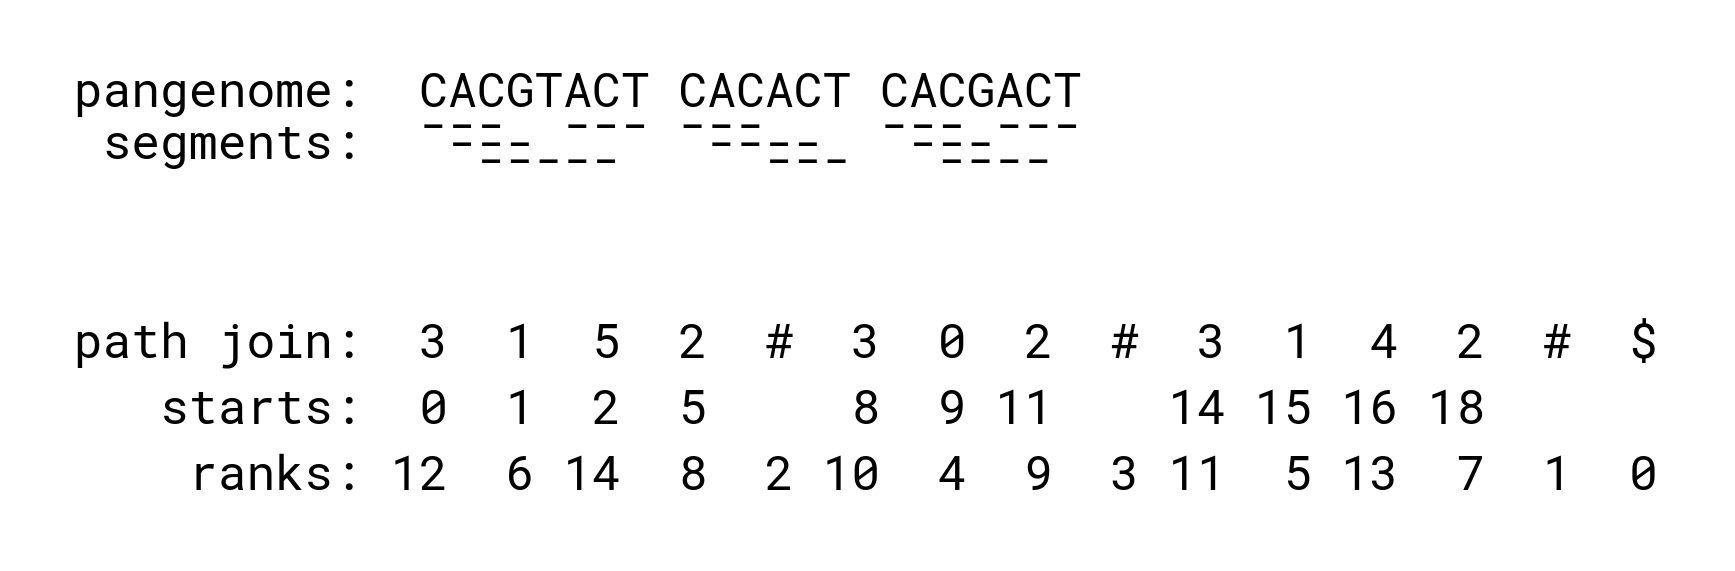
\includegraphics[width=\linewidth]{images/path_join.png}
    \caption{}
    \label{fig:path_join}
\end{figure}

\begin{table}
    \caption{Segment table}
    \label{tab:segment}
    \begin{tabular}{rrll}
        \toprule
        id & length & starts & right context ranks \\
        \midrule
        0 & 4 & 14          & 9         \\
        1 & 3 & 23, 2       & 13, 14    \\
        2 & 5 & 28, 8, 17   & 1, 2, 3   \\
        3 & 3 & 12, 21, 0   & 4, 5, 6   \\
        4 & 4 & 25          & 7         \\
        5 & 5 & 4           & 8         \\
        \bottomrule
    \end{tabular}
\end{table}




\subsection{Iterating suffix array}
With the previous tables in memory, we have all we need to generate the suffix
array entries.
Due to the prefix-freeness of the segments and the construction of the segment join
we can ignore all characters after the first delimiter of $\texttt{suffix}[i..]$.
Then, each row in the suffix table represents a suffix of a particular segment.

There are three cases where a letter at position $SA[i]$ can occur in these suffix segments:
\begin{itemize}
    \item it is a separator or the sentinel
    \item it is at the end of a segment inside the trigger part
    \item it is part of the segment outside the trigger part, separator and sentinel
\end{itemize}

In the first case, there is no corresponding position in the original pangenome,
therefore we can skip these rows of the suffix table.
% We can skip the first $n+1$ rows of the suffix table, because these suffixes
% do not yield any suffix array entry.

In the second case, the position is inside the trigger string.
Since the possitions inside the triggers are represented twice, once at the end
of a segment a second time at the beginning of the following segment, we need
to choose when to report them.
A natural choice is to report positions at the beginning of a segment and ignore
positions at the end.
Here we note that this choice also plays nicely with the previous choice of sentinel
characters, since ignoring last $k$ characters will result in not printing
sentinels either.
In conclusion, if the length of a current segment suffix is smaller or equal to
the size of the trigger words, we skip the row similarly as in the previous case.

Finaly, in the last case we report the positions.
The last case will partition the suffix table into the blocks of the same suffixes.
As an example consider the rows 20 and 21, which together for a single block.
All other blocks in the example consist of single rows and therefore we call them singletons.

This partitioning leads to three cases (from simplest to hardest):
\begin{itemize}
    \item A singleton block, occuring only once in the whole pangenome
    \item A singleton block, repeating several times in the pangenome
    \item A non-singleton block
\end{itemize}

In the case of a singleton block with only a single occurence we need to report only a single suffix array entry.
Given the row index $i$, this entry can be calculated with the following equation:

\begin{equation}
    \label{eq:sa_entry}
    \texttt{SA entry} = \texttt{starts}[\texttt{ID}[i]] + \texttt{pos}[i]
\end{equation}

As an example, consider the row $13$ in the Suffix Table (\ref{tab:suffix}), the first row yielding a SA value.
It's segment ID is $0$ and from the Segment Table (\ref{tab:segment}) we see that there is only one occurence of segment $0$ and it starts at position $9$ in the pangenome.
The offset from the start of a segment $\texttt{pos}[13]$ is $0$.
This yields the first entry of a suffix array $9 + 0 = 9$ corresponding to the lexicographically smallest suffix $P[9..] = \texttt{ACACT}$.

The second, slightly more complex case is a singleton block with several occurences in the pangenome.
For this case, we need to report as many suffix array entries as the number of occurences.
Because the starting segment positions in the Segment Table (\ref{tab:segment}) are sorted based on their right context rank, we can iterate through these starting positions and apply Equation \ref{eq:sa_entry} to each of them.

As an example, consider the row $14$ in the Suffix Table (\ref{tab:suffix}).
This suffix occurs twice in the pangenome in segments starting at positions $15$ and $1$.
Since the offset from the start of a segment $\texttt{pos}[14]$ is $0$, we report a suffix array entry $15 + 0 = 15$ and $1 + 0 = 1$, corresponding to the suffixes $P[15..] = \texttt{ACGACT}$ and $P[1..] = \texttt{ACGTACT}$.

In the last case, we have a non-singleton block with suffixes of several segments, possibly with multiple occurences.
These suffixes represent the same substring of the original pangenome.
Here, we report a suffix array entry for each occurence of the substring in the pangenome.
To identify which entry is the first, we need to find the starting position with the smallest right context rank.
Because the ranks are sorted, this procedure is similar to the merging phase of a merge sort.
To iterate through all suffix array entries in the block, we therefore always identify the segment start with the next smallest right context rank and apply Equation \ref{eq:sa_entry} to this segment start.

As an example, consider the block at rows $[20..21]$ in the Suffix Table (\ref{tab:suffix}).
The relevant segment IDs are $0$ and $3$, with segment starts at positions $9$, $8$, $14$ and $0$.
The right context ranks from smallest to highest are $4, 5, 6, 9$ with the corresponding segment starts $8, 14, 0, 9$.
Applying Equation \ref{eq:sa_entry} to these segment starts yields a suffix array entries $8 + 0 = 8$, $14 + 0 = 14$, $0 + 0 = 0$ and $9 + 1 = 10$, representing pangenome suffixes $P[8..] = \texttt{CACACT}$, $P[14..] = \texttt{CACGACT}$, $P[0..] = \texttt{CACGTACT}$, and $P[10..] = \texttt{CACT}$.

\section{Related work}
There are several proposed data structures implicitly relying on the structure
of prefix-free graphs.

Rpair: rescaling repair with rsync \cite{2019gagie}
Prefix-free parsing for building big BWTs \cite{2019boucher}
MONI and r-index \cite{rossi2022moni,gagie2020fully}
Prefix-free Wheeler graphs \cite{2022pfwg}
MARIA \cite{2022maria}

All of these works implement their own version of prefix-free graphs.
We argue that separating prefix-free graphs as a standalone data structure can
bring several benefits:

\begin{itemize}
    \item reduce the complexity of the presentation
    \item allowing for better optimization of algorithms related to prefix-free graphs
    \item supporting the theoretical research by clearly deliminating the relevant terms
    \item allowing to bring prefix-free graphs closer to the biological data
\end{itemize}

Related to the last point, we remark that a possible future research can be in
the proper choice of trigger words.
As an example, we used stop codons in our experiments.
This could create prefix-free graphs capturing some biologically relevant phenomena.
Other options are recombination hotspots, highly repetitive elements, different
binding sites and sites with increased breakage.

\section{Results}
We implemented the prefix-free graphs package in rust programming language.
There are two binary crates and one library crate included in the package.
Binary crates serve the purpose of creating prefix-free graphs from FASTA and from GFA formats.
Library crate provides an interface for working with the prefix-free graphs,
mainly an iterator of suffix array in sublinear space and linear time.

The binary crates are fasta2pfg and gfa2pfg with usage:
\begin{minted}{bash}
fasta2pfg -t triggers.txt < pangenome.fna > pfg.gfa

gfa2pfg -t triggers.txt < pangenome.gfa > pfg.gfa
\end{minted}

The library can be used from within rust programming language as follows:

\begin{minted}{rust}
let pfg = PFG::load("pfg.gfa");

for (i, sa_i) in pfg.iter().enumerate() {
    println!("{}\t{}", i, sa_i);
}
\end{minted}

\section{Discussion}

\begin{acknowledgments}
    Thanks to Alessia and Askar for their encouragement while developing prefix-free graphs.
\end{acknowledgments}

\bibliography{sources}

\appendix

\section{Online Resources}

The sources for the prefix-free graphs are available via
\begin{itemize}
\item \href{https://github.com/andynet/pfg}{GitHub}.
\end{itemize}

\end{document}

